\section{Study Area}
\label{sec:study-area}

The GeoSoil-Cuba study area is located in Jaruco,
Mayabeque Province, western Cuba. The Area of Interest
(AOI) covers approximately
\SI{178.47}{\square\kilo\metre} and encompasses
agricultural landscapes, natural and semi-natural
vegetation, and the Mampostón reservoir (\Cref{fig:study_area_location}). Administrative boundaries were obtained from
the GADM database, version 4.1, using the
Cuba GeoPackage dataset
(\texttt{gadm41\_CUB.gpkg})
\parencite{gadm2022}. Both location maps were prepared in QGIS.
Cartographic elements, including coordinate
grids, scale bars, north arrows, and geographic
labels, were configured using the QGIS
print layout. 

This geographic setting provides a basis for integrating
historical soil cartography, land-cover information,
and satellite-derived vegetation observations.

\begin{figure}[htbp]
	\centering
	
	% (a) Geographic location of Mayabeque, Cuba
	\begin{subfigure}[t]{0.48\textwidth}
		\centering
		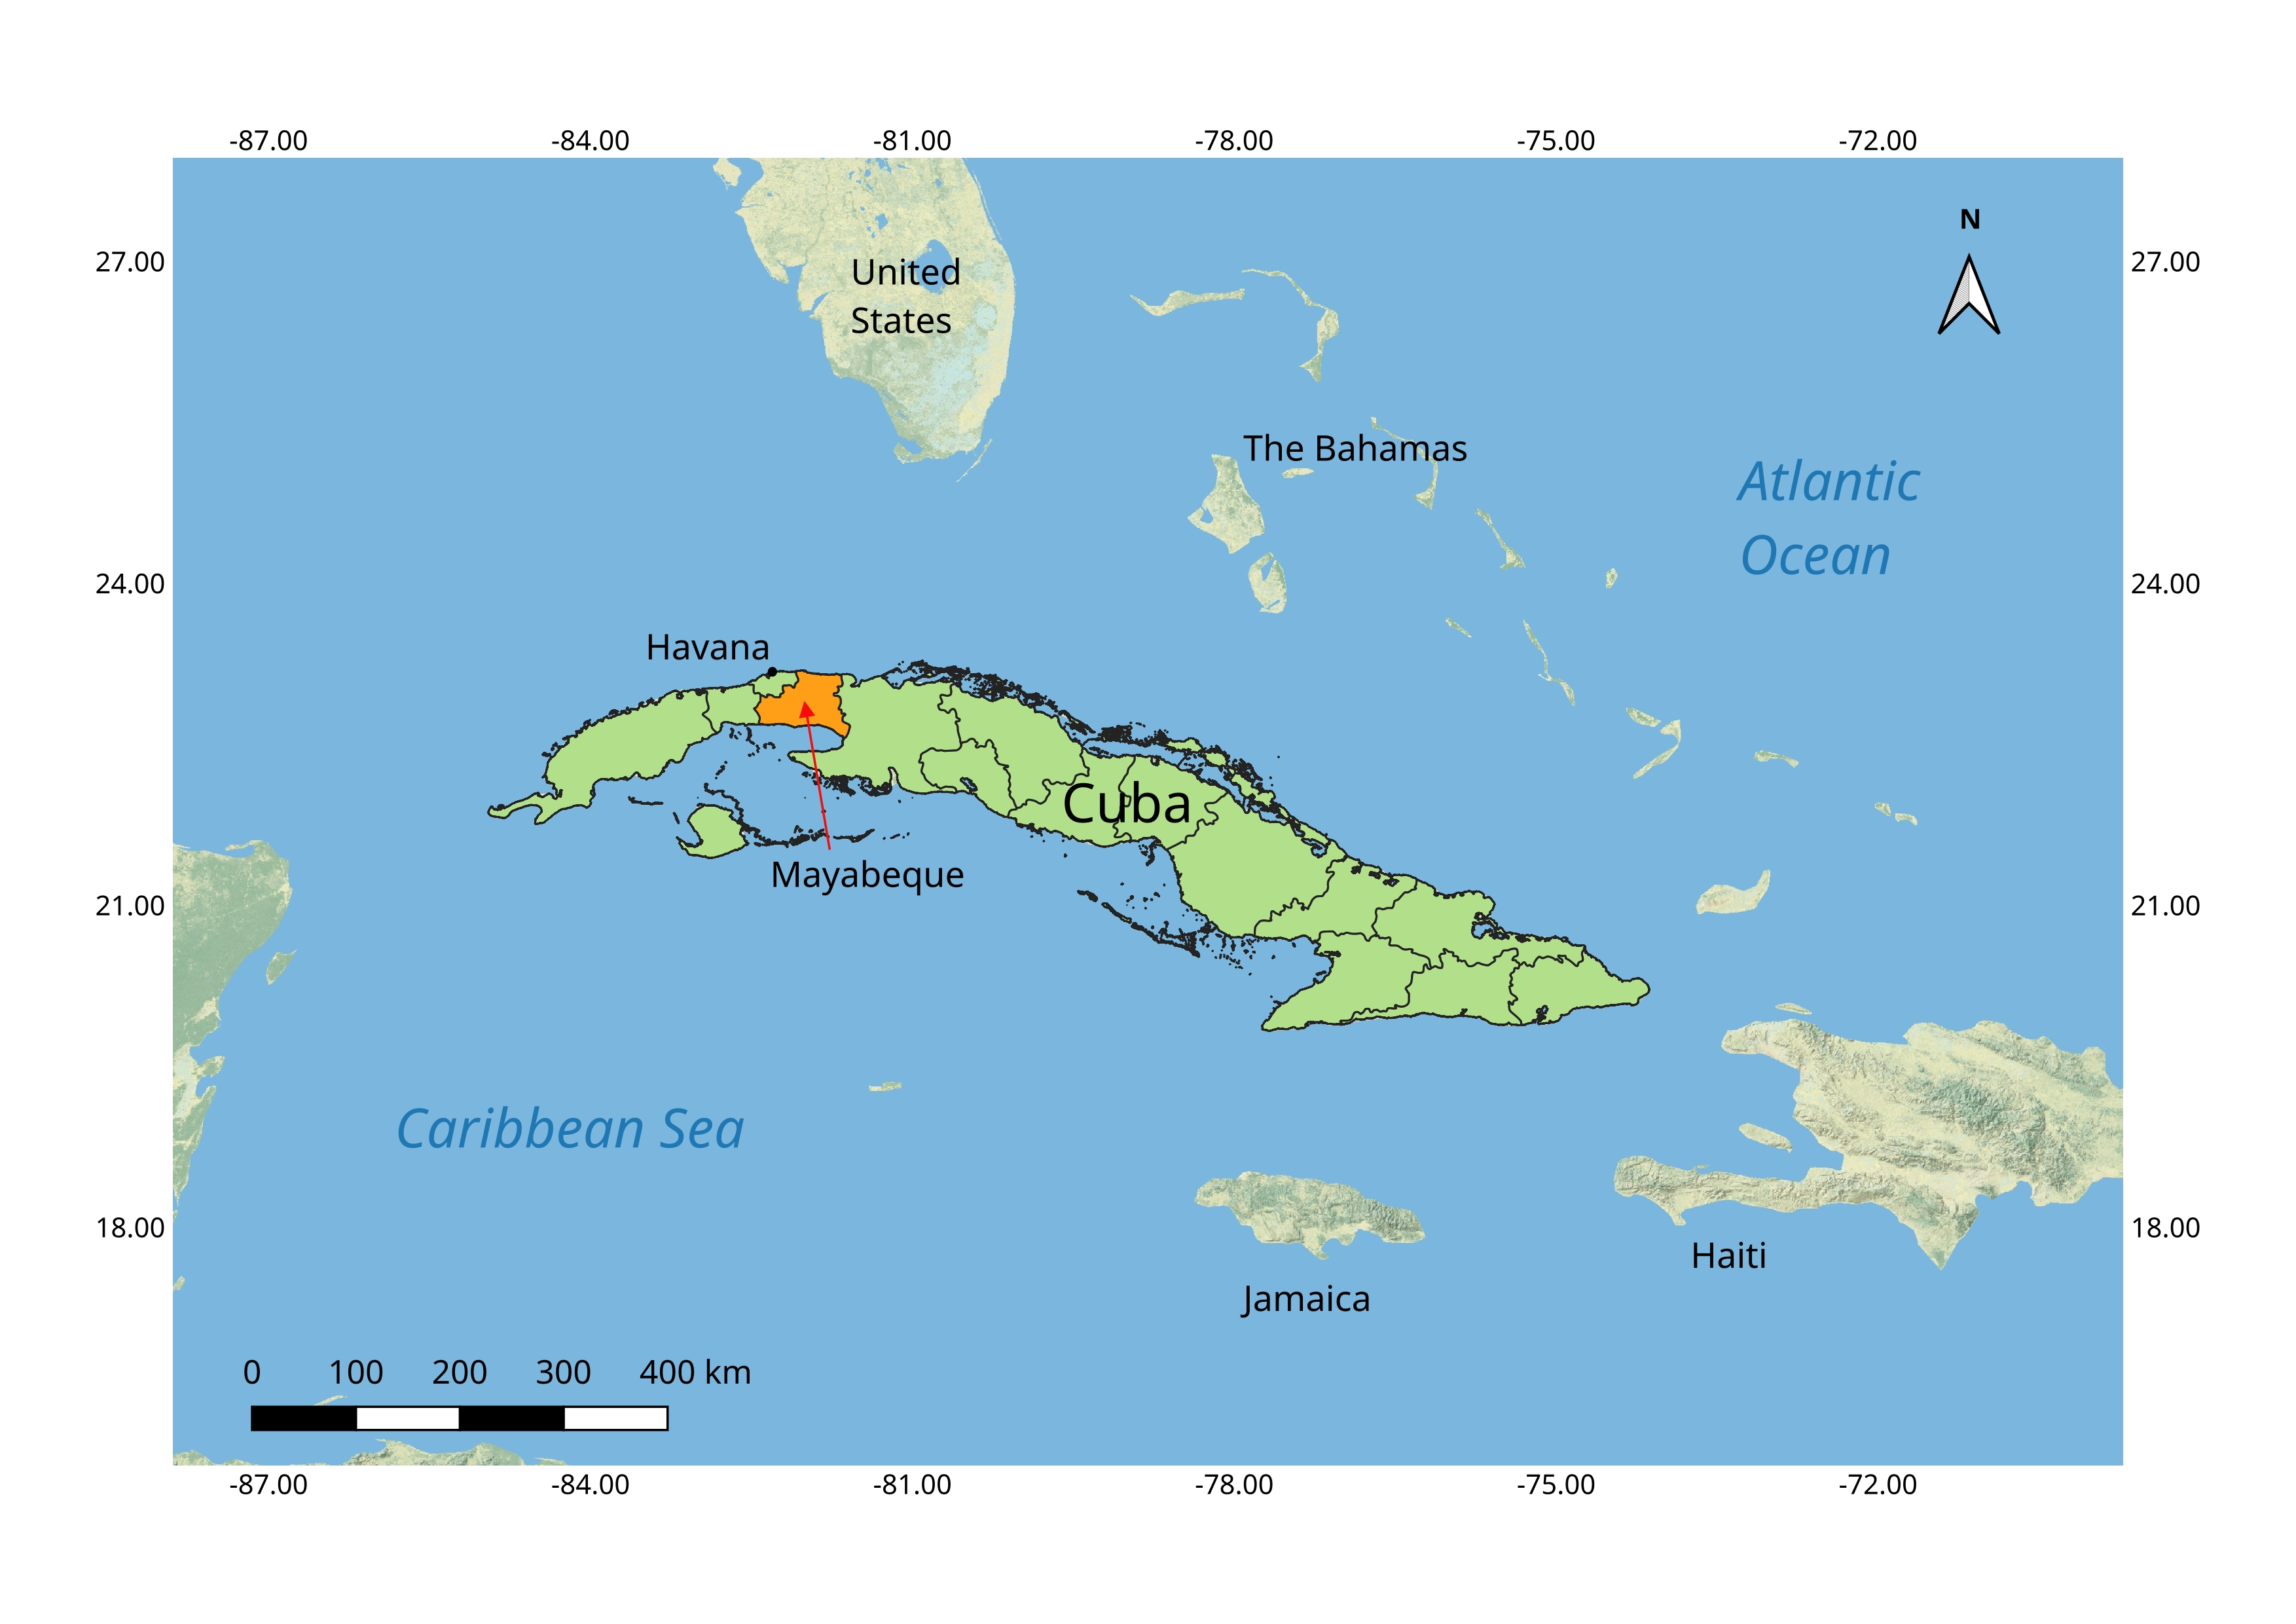
\includegraphics[
		width=\linewidth,
		height=5.5cm,
		keepaspectratio
		]{../figures/caribe-cuba.jpg}
		
		\caption{Geographic location of Mayabeque Province, Cuba.}
		\label{fig:mayabeque_location}
	\end{subfigure}
	\hfill
	% (b) Study area in Jaruco, Mayabeque
	\begin{subfigure}[t]{0.48\textwidth}
		\centering
		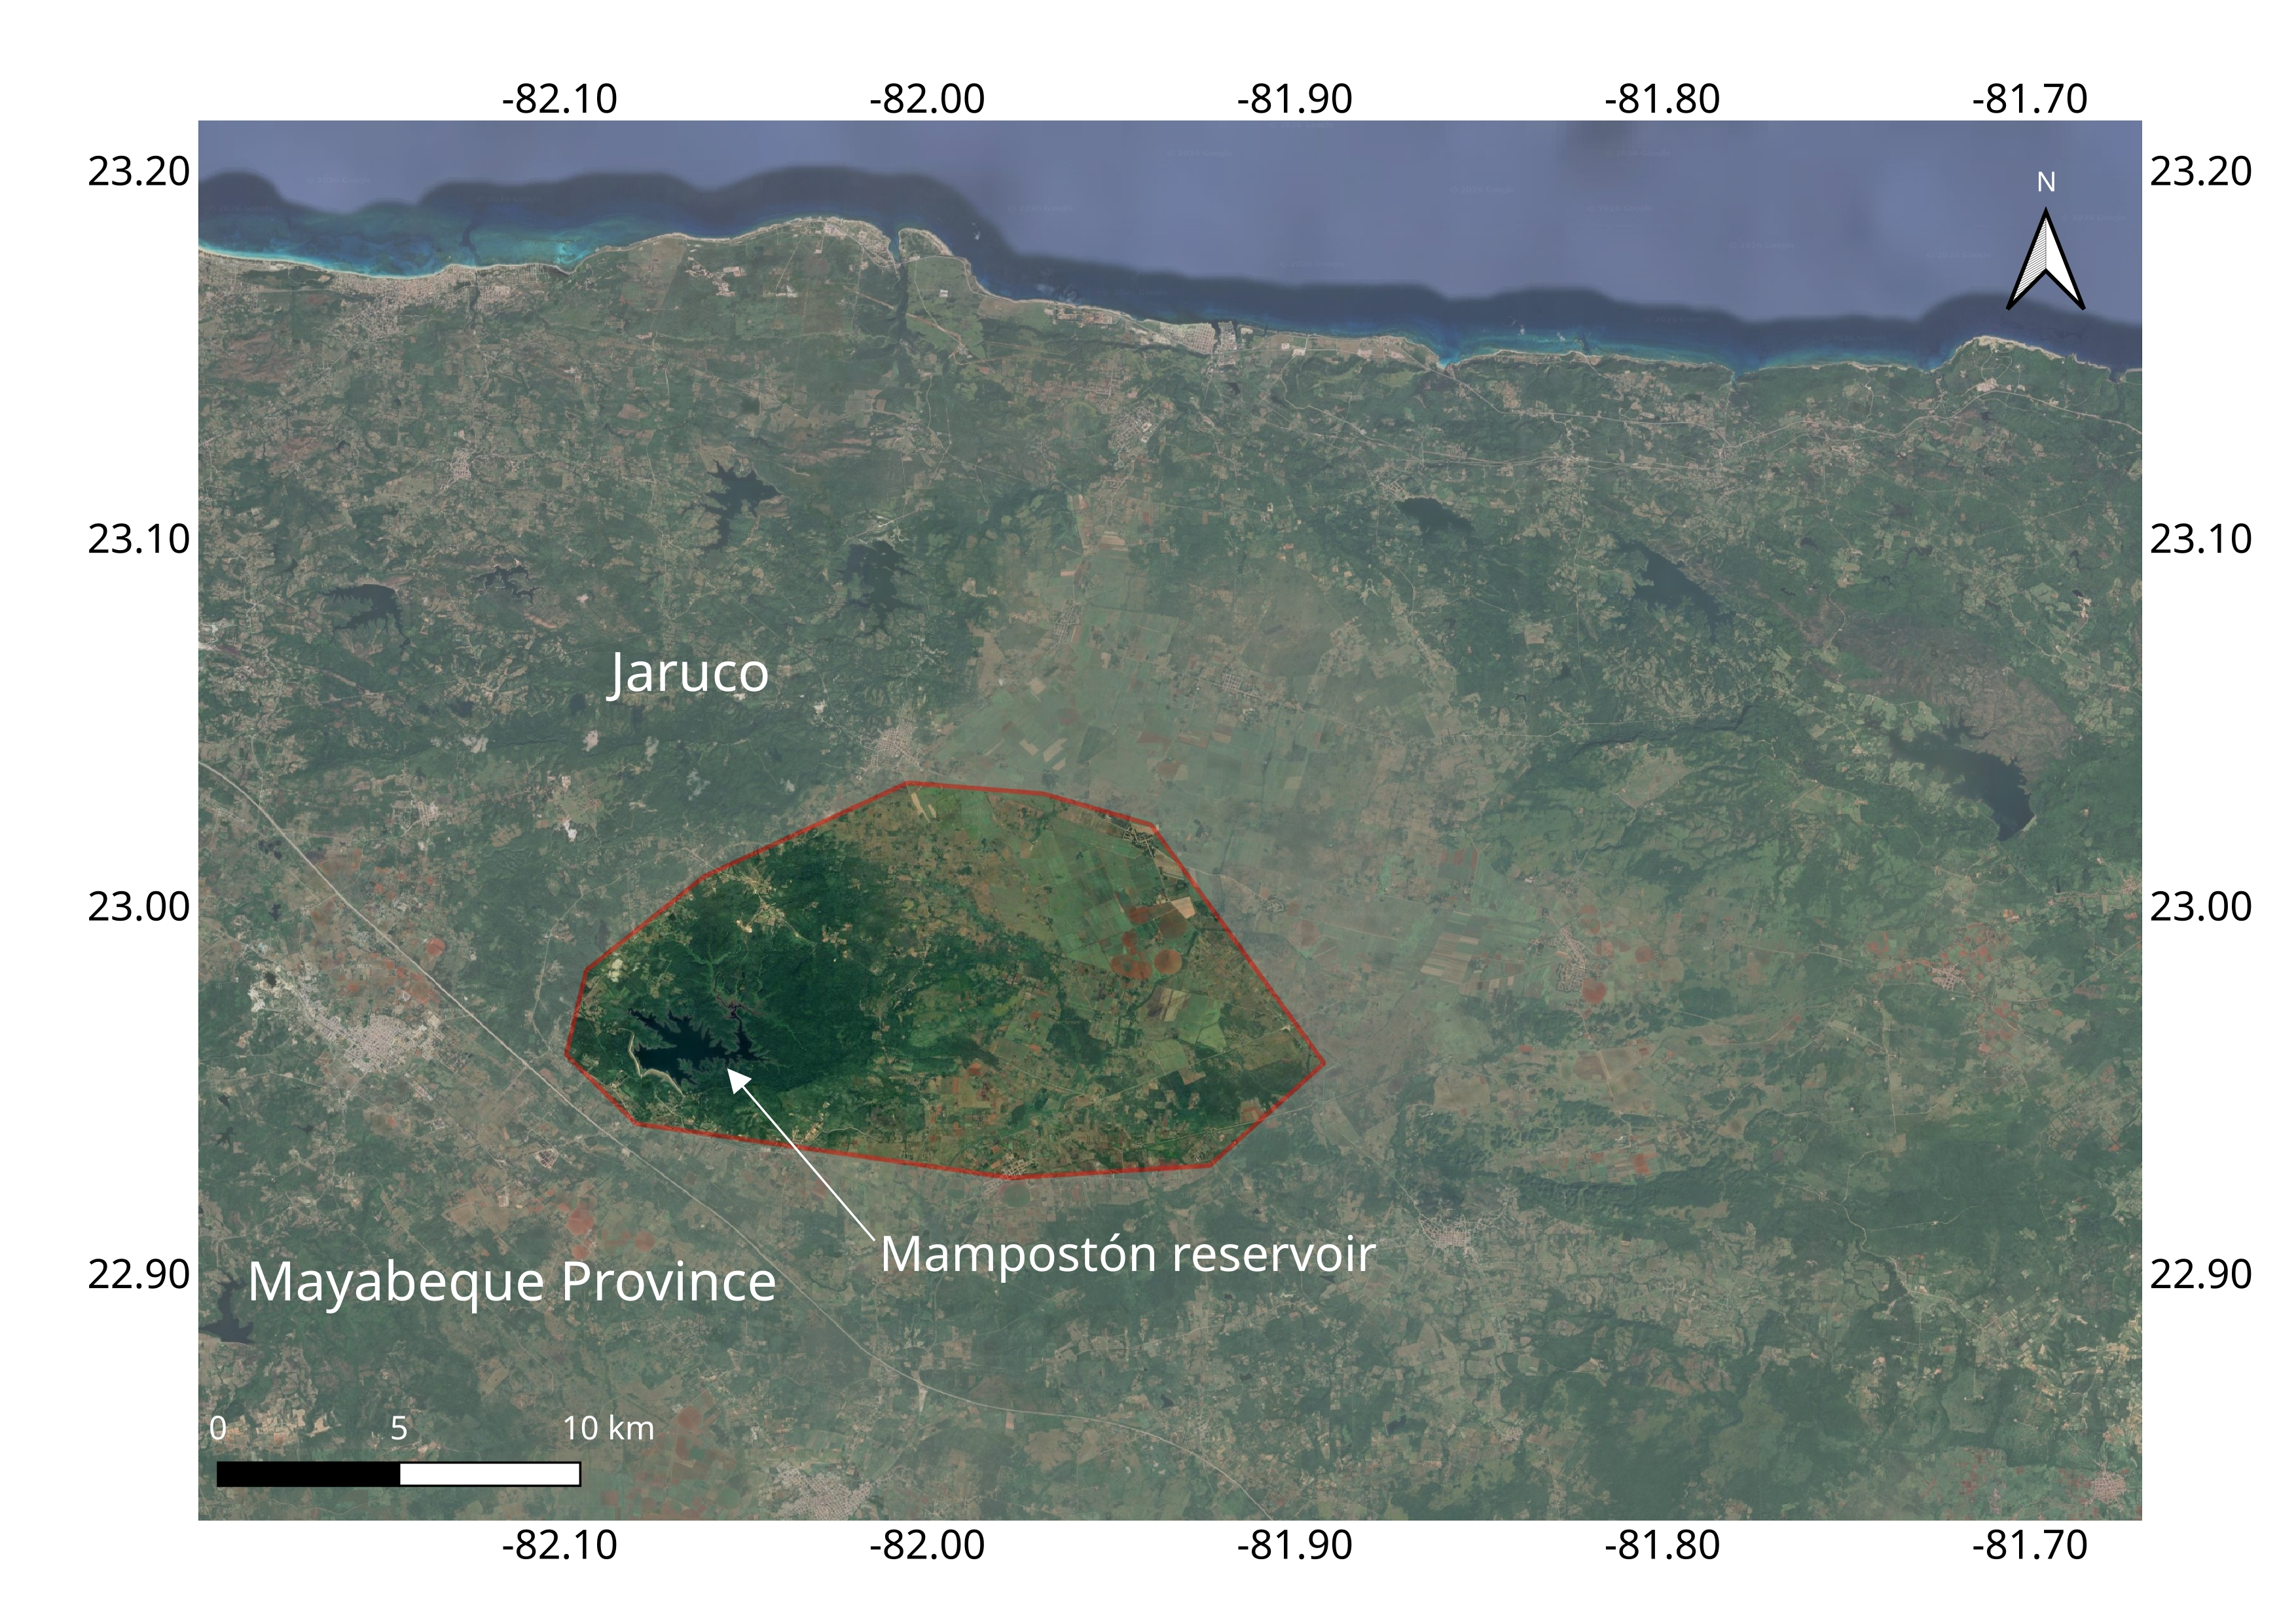
\includegraphics[
		width=\linewidth,
		height=5.5cm,
		keepaspectratio
		]{../figures/escala-mayabeque.jpg}
		
		\caption{Study area in Jaruco, Mayabeque Province.}
		\label{fig:jaruco_study_area}
	\end{subfigure}
	
	\caption{
		Geographic location of the study area:
		(a) Mayabeque Province within Cuba and
		(b) study area in Jaruco Municipality,
		Mayabeque Province.
		Maps prepared by the author using QGIS.
		Administrative boundaries derived from
		GADM version 4.1~\parencite{gadm2022}.
	}
	\label{fig:study_area_location}
\end{figure}

The AOI was defined using a geographic boundary
provided in Keyhole Markup Language (KML) format.
The original boundary uses the WGS 84 geographic
coordinate reference system (EPSG:4326). Its
approximate geographic extent ranges from
\ang{22.92585} to \ang{23.03332} north latitude
and from \ang{-82.09837} to \ang{-81.89215}
longitude.

For spatial analyses involving the historical soil
map, the AOI was transformed to NAD27 / Cuba Norte
(EPSG:3795), the projected coordinate reference
system used by the source cartographic dataset.
This transformation facilitates spatial
intersection, clipping, and area calculations
within a common coordinate reference system.

The Mampostón reservoir is a relevant geographic
feature within the AOI. Because open-water surfaces
are not expected to be represented by terrestrial
soil mapping units, their presence must be
considered when assessing soil-map coverage.
Accordingly, areas without mapped soil information
must be distinguished from water surfaces and
from other gaps that may remain within the
terrestrial analysis area.

Within the broader AOI, a unified agricultural
region was delineated for the regional NDVI
time-series analysis. A complementary analysis
examined vegetation-index observations within
three locally verified potato fields, represented
by sampling polygons digitized in QGIS. These
spatial units support different analytical
purposes: the AOI provides the overall context
for soil and land-cover integration, whereas the
agricultural region and field samples support
the examination of vegetation variability at
regional and field scales, respectively.

The study area was selected to evaluate the
integration and spatial consistency of existing
soil cartographic information, land-cover
classifications, and satellite observations.
The combined analyses provide a basis for
assessing soil-map coverage and examining
temporal vegetation-index patterns without
assuming that observed NDVI differences are
caused by soil properties or agricultural
management.

